% $Header: /cvsroot/latex-beamer/latex-beamer/solutions/conference-talks/conference-ornate-20min.en.tex,v 1.6 2004/10/07 20:53:08 tantau Exp $

\documentclass{beamer}

% This file is a solution template for:

% - Talk at a conference/colloquium.
% - Talk length is about 20min.
% - Style is ornate.



% Copyright 2004 by Till Tantau <tantau@users.sourceforge.net>.
%
% In principle, this file can be redistributed and/or modified under
% the terms of the GNU Public License, version 2.
%
% However, this file is supposed to be a template to be modified
% for your own needs. For this reason, if you use this file as a
% template and not specifically distribute it as part of a another
% package/program, I grant the extra permission to freely copy and
% modify this file as you see fit and even to delete this copyright
% notice.


\mode<presentation>
{
%  \usetheme{Warsaw}
%  \usetheme{Boadilla}
%  \usetheme{Goettingen}
%  \usetheme{Hannover}
%  \usetheme{Madrid}
%  \usetheme{Marburg}
%  \usetheme{Montpellier}
%  \usetheme{Pittsburgh}
  \usetheme{Hawke}
  % or ...

  \setbeamercovered{transparent}
  % or whatever (possibly just delete it)
}


\usepackage[english]{babel}
% or whatever

\usepackage[latin1]{inputenc}
% or whatever

\usepackage{times}
\usepackage[T1]{fontenc}
% Or whatever. Note that the encoding and the font should match. If T1
% does not look nice, try deleting the line with the fontenc.

\usepackage{multimedia}


%%%%%%
% My Commands
%%%%%%

\usepackage{SULectureMathsSlides}

\newcommand{\ml}{{\sc matlab}}
\newcommand{\bfm}[1]{{\boldsymbol{#1}}}
%\newcommand{\bx}{\bfm{x}}
%\newcommand{\bb}{\bfm{b}}

%%%%

\title[Lecture 27] % (optional, use only with long paper titles)
{Lecture 27 - Eigenvalues and the power method}

% \subtitle
% {Include Only If Paper Has a Subtitle}

\author[I.~Hawke] % (optional, use only with lots of authors)
{I.~Hawke}
% - Give the names in the same order as the appear in the paper.
% - Use the \inst{?} command only if the authors have different
%   affiliation.

\institute[University of Southampton] % (optional, but mostly needed)
{
%  \inst{1}%
  School of Mathematics, \\
  University of Southampton, UK
}
% - Use the \inst command only if there are several affiliations.
% - Keep it simple, no one is interested in your street address.

\date[Semester 1] % (optional, should be abbreviation of conference name)
{MATH3018/6141, Semester 1}
% - Either use conference name or its abbreviation.
% - Not really informative to the audience, more for people (including
%   yourself) who are reading the slides online

\subject{Numerical methods}
% This is only inserted into the PDF information catalog. Can be left
% out.



% If you have a file called "university-logo-filename.xxx", where xxx
% is a graphic format that can be processed by latex or pdflatex,
% resp., then you can add a logo as follows:

\pgfdeclareimage[height=0.5cm]{university-logo}{mathematics_7469}
\logo{\pgfuseimage{university-logo}}



% Delete this, if you do not want the table of contents to pop up at
% the beginning of each subsection:
%  \AtBeginSubsection[]
%  {
%    \begin{frame}<beamer>
%      \frametitle{Outline}
%      \tableofcontents[currentsection,currentsubsection]
%    \end{frame}
%  }
\AtBeginSection[]
{
  \begin{frame}<beamer>
    \frametitle{Outline}
    \tableofcontents[currentsection]
  \end{frame}
}


% If you wish to uncover everything in a step-wise fashion, uncomment
% the following command:

%\beamerdefaultoverlayspecification{<+->}


\begin{document}

\begin{frame}
  \titlepage
\end{frame}


\section{Eigenvalues}

\subsection{Revision}

\begin{frame}
  \frametitle{Eigenvalues - revision}

  Eigenvalues, $\lambda$ and their corresponding eigenvectors
  $\boldsymbol{u}$ are non-zero solutions to the linear system
  %
  \begin{equation*}
    A\boldsymbol{u} = \lambda \boldsymbol{u}.
  \end{equation*}
  %
  \pause
  Matrix eigenthings often important: e.g. resonant modes of system, or defining spectral radius $\varrho(M) = \max | \lambda(M) |$ which encodes e.g.\ convergence of iterative schemes for linear systems.

\end{frame}

\subsection{Eigenvalues}

\begin{frame}
  \frametitle{Eigenvalues and polynomials}

  Standard definition of eigenvalues: the $n$ roots of
  the \emph{characteristic polynomial}
  \begin{equation*}
    \det ( A - \lambda I) = 0.
  \end{equation*}
  Could compute roots e.g.\ by nonlinear root finding. \pause

  \vspace{1ex}

  There are two essential problems with this:
  \begin{enumerate}
  \item Frequently do not need all eigenvalues, but only the largest
    one(s). Computing all, and then sorting, excessively
    expensive. \pause
  \item Polynomials may be \emph{badly conditioned}: a small change in
    the coefficients leads to a large change in the roots.
  \end{enumerate} \pause

  \vspace{1ex}

  A $1\%$ change in the last coefficient leads to massive changes for
  \begin{equation*}
    p(z) = -120 + 274 z - 225 z^2 + 85 z^3 -15 z^4 + z^5;
  \end{equation*}
  the roots $(4, 5)$ become $(4.580 \pm 0.966 \sqrt{-1})$.

\end{frame}


\subsection{The power method}

\begin{frame}
  \frametitle{The power method}

  Want to compute largest eigenvalue without relying
  on characteristic polynomial. Hint from first computer lab:
  \begin{center}
    \includegraphics<1|handout:0>[height=0.7\textheight]{figures/Power1}
    \includegraphics<2|handout:0>[height=0.7\textheight]{figures/Power2}
    \includegraphics<3|handout:0>[height=0.7\textheight]{figures/Power3}
    \includegraphics<4>[height=0.7\textheight]{figures/Power4}
  \end{center}

\end{frame}

\begin{frame}
  \frametitle{The power method: basis vectors}

  Key to power method: \emph{assumption} that eigenvectors $\{
  \bfm{u}_n \}$ form a basis of ${\mathbb C}^n$.  If true, repeated
  action of $A$ on \emph{generic} vector $\bfm{x}$ picks out
  eigenvector with largest eigenvalue.  \pause

  Specifically, construct sequence of vectors $\{ \bx^{(n)}
  \}$. Initial guess $\bx^{(0)}$ (nearly) arbitrary, members of
  sequence are
  \begin{equation*}
    \bx^{(k)} = A^k \bx^{(0)}.
  \end{equation*} \pause

  Writing initial guess in terms of basis of eigenvectors shows
  \begin{equation*}
    \bx^{(0)} = \sum_{j=1}^n a_j \bfm{u}_j \, \implies \,
    \bx^{(k)} = \lambda_1^k \left[ a_1 \bfm{u}_1 + \left(
        \frac{\lambda_2}{\lambda_1} \right)^{\mathclap{k}} a_2 \bfm{u}_2 + \dots + \left(
        \frac{\lambda_n}{\lambda_1} \right)^{\mathclap{k}} a_n \bfm{u}_n \right].
  \end{equation*} \pause
  %
  If $| \lambda_j / \lambda_1 | < 1 \quad \forall j > 1$ then the
  first term dominates.

\end{frame}

\begin{frame}
  \frametitle{Caveats}

  Some points have been glossed over:
  \begin{enumerate}
  \item Have assumed \emph{unique} eigenvalue of maximum
    modulus. \pause
  \item Have assumed the eigenvectors exist and are linearly
    independent. \pause This is necessary to have a
    basis of eigenvectors. \pause
  \item Have assumed the initial guess $\bx^{(0)}$ has a nonzero
    component in the direction of eigenvector $\bfm{u}_1$; i.e.\
    if
    \begin{equation*}
      \bx^{(0)} = \sum_{j=1}^n a_j \bfm{u}_j \quad \implies \quad a_1 \neq 0.
    \end{equation*} \pause
    %
    Not a major problem: repeated numerical operations have floating
    point error, so $a_1$ will never be \emph{precisely} zero.  Method
    converges faster the closer that $\bx^{(0)}$ is aligned with
    $\bfm{u}_1$.
  \end{enumerate}

\end{frame}

\begin{frame}
  \frametitle{Error terms}

  Can write the iterative method given by the power method as
  \begin{equation*}
    \bx^{(k)} = \lambda_1^k \left( a_1 \bfm{u}_1 + \epsilon^{(k)} \right)
  \end{equation*}
  where the term
  \begin{equation*}
    \epsilon^{(k)} \equiv \sum_{j=2}^n \left(
      \frac{\lambda_j}{\lambda_1} \right)^k a_j \bfm{u}_j
  \end{equation*}
  is expected to vanish in the limit. \pause Explicitly,
   \begin{equation*}
     \| \epsilon^{(k)} \| = {\cal O} \left( \left|
       \frac{\lambda_j}{\lambda_1} \right|^k \right)
   \xrightarrow[k \rightarrow \infty]{} 0.
   \end{equation*} \pause

   \vspace{1ex}

   In general expect the ``error term'' at each step to diminish by
   $|\lambda_2 / \lambda_1|$, giving linear convergence, as seen
   later.

\end{frame}


\subsection{Algorithm}


\begin{frame}
  \frametitle{Algorithm: 1}

  The simplest (and not fully correct) algorithm defines the ratio
  \begin{equation*}
    r_k = \frac{\| \bx^{(k+1)} \|}{\| \bx^{(k)} \|} = |\lambda_1|
    \frac{\| a_1 \bfm{u}_1 + \epsilon^{(k+1)} \|}{\| a_1 \bfm{u}_1 +
      \epsilon^{(k)} \|}.
  \end{equation*} \pause
  From the convergence of the ``error term'' we then have that
  \begin{equation*}
    \lim_{k\rightarrow\infty} r_k = | \lambda_1 |.
  \end{equation*} \pause

  Algorithm is impractical: unless $\lambda_1$ is \emph{extremely}
  close to 1, iterates diverge to infinity or zero, spoiling
  accuracy. \pause Instead redefine members of sequence to
  have unit norm \emph{after} computing the ratio $r_k$:
  \begin{enumerate}
  \item Pick $\bx^{(0)}$ such that $\|\bx^{(0)}\|=1$.
  \item For each $k$ compute $\bx^{(k+1)} = A \bx^{(k)}$.
  \item Compute $r_k = \| \bx^{(k+1)} \|$ (as $\| \bx^{(k)} \| = 1$).
  \item Re-normalize $\bx^{(k+1)}$. Repeat from (2).
  \end{enumerate}

\end{frame}

\begin{frame}[fragile]
  \frametitle{Example}

  The core of a simple Python script for the power method:
\begin{verbatim}
for k in range(1, niterations_max):
    xn[:,k-1] = xn[:,k-1]/numpy.linalg.norm(xn[:,k-1])
    xn[:,k] = numpy.linalg.dot(A, xn[:, k-1])
    rn[k] = numpy.linalg.norm(xn[:,k])/numpy.linalg.norm(xn[:,k-1])
    if abs(rn[k] - rn[k-1]) < tol:
        break
lambda = rn[k]
\end{verbatim}

\end{frame}

\begin{frame}
  \frametitle{Example 2}

  \begin{center}
    \includegraphics<1|handout:1>[height=0.85\textheight]{figures/PowerSimple1}
    \includegraphics<2|handout:2>[height=0.85\textheight]{figures/PowerSimple2}
  \end{center}

\end{frame}


\subsection{Phase information}


\begin{frame}
  \frametitle{Beyond the absolute value}

  Although $\max |\lambda|$ useful, straightforward to modify power
  method to compute actual full value. \pause

  \vspace{1ex}

  The eigenvalue is complex (in general), so in computing just the
  \emph{modulus} have lost information about the \emph{phase}.  Phase
  information lost when norms are computed. So replace the norms with
  a different \emph{linear} functional $\phi: {\mathbb C}^n
  \rightarrow {\mathbb R}$. \pause

  \vspace{1ex}

  Then have
  \begin{equation*}
    r_k = \frac{\phi(\bx^{(k+1)})}{\phi(\bx^{(k)})} = \lambda_1
    \frac{ a_1 \phi(\bfm{u}_1) + \phi(\epsilon^{(k+1)})}{ a_1 \phi( \bfm{u}_1) +
      \phi(\epsilon^{(k)})};
  \end{equation*}
  depends on the linearity of $\phi$. In the limit get full eigenvalue
  $\lambda_1$. \pause

  \vspace{1ex}

  One possible choice for $\phi$ is to simply sum the components of
  $\bx$. In all cases care must be taken to avoid dividing by zero.

\end{frame}

\begin{frame}
  \frametitle{Example}

  \begin{columns}
    \begin{column}{0.35\textwidth}
      Apply the power method to the matrix
      \begin{equation*}
        A =
        \begin{pmatrix}
          1 & 2 & 3 \\
          4 & 5 & 6 \\
          7 & 8 & 0
        \end{pmatrix}.
      \end{equation*}
      The result converges linearly to find $\lambda = 12.1229$.

      \vspace{1ex}

      Identical convergence is seen for $-A$.
    \end{column}
    \begin{column}{0.65\textwidth}
      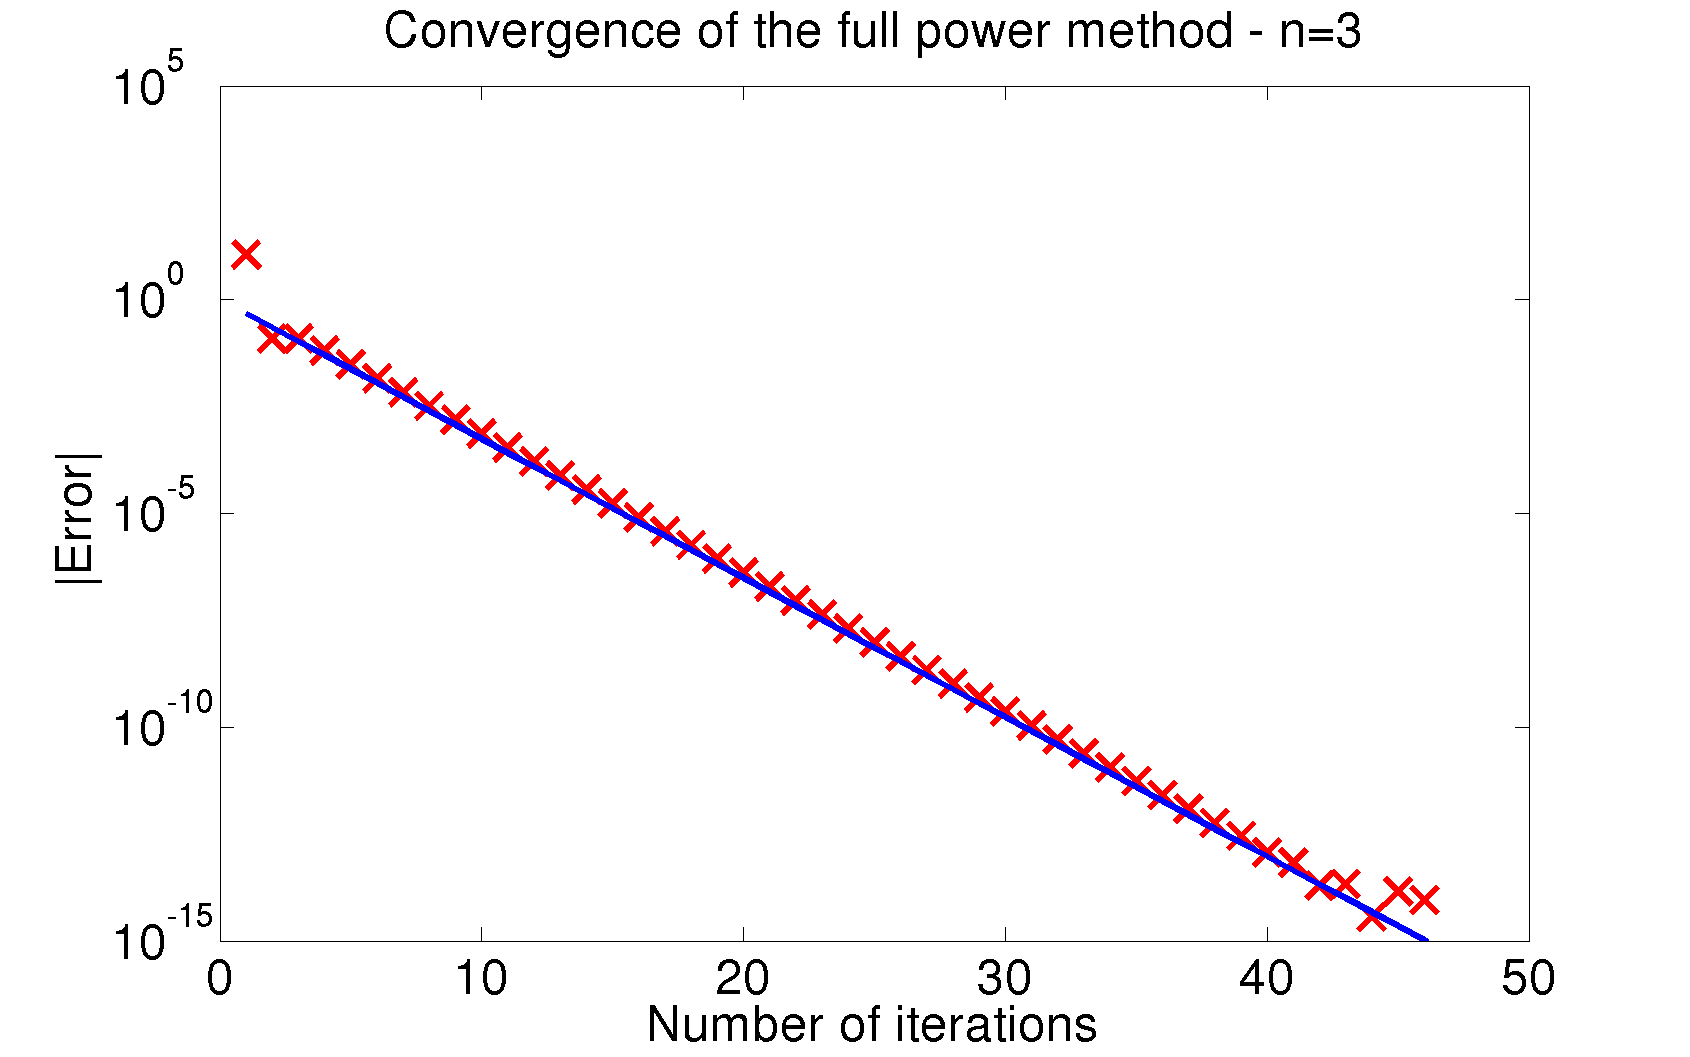
\includegraphics[width=\textwidth]{figures/PowerFull1}
    \end{column}
  \end{columns}
\end{frame}


\subsection{Convergence}


\begin{frame}
  \frametitle{Rate of convergence}

  Look at behaviour near solution using Taylor's theorem.

  \vspace{1ex}

  Start by defining $\mu = \lambda_2 / \lambda_1$.
  Use as ``small parameter'' in expansion. Note that
  \begin{equation*}
    \left| \frac{\lambda_j}{\lambda_1} \right|  < |\mu| \quad \forall
    j > 2.
  \end{equation*} \pause
  %
  Rewrite ratio as
  \begin{equation*}
    r_k =  \lambda_1
    \frac{ a_1 \phi(\bfm{u}_1) + \phi(\epsilon^{(k+1)})}{ a_1
      \phi( \bfm{u}_1) + \phi(\epsilon^{(k)})} = \lambda_1 \left[
      1 - \phi (\epsilon^{(k)}) \right] + {\cal O} (\mu^{k+1}).
  \end{equation*} \pause
  %
  The relative error is then
  \begin{equation*}
    E^{(k)} = \left| \frac{r_k - \lambda_1}{\lambda_1} \right|
    = \left| \phi( \epsilon^{(k)} ) \right|  + {\cal O}
    (\mu^{k+1})
    = c_k \mu^k.
  \end{equation*}
  %
  Hence we have a linear decrease at each stage of a factor $\mu$.

\end{frame}


\begin{frame}
  \frametitle{Example revisited}

  \begin{columns}
    \begin{column}{0.35\textwidth}
      The matrix
      \begin{equation*}
        A =
        \begin{pmatrix}
          1 & 2 & 3 \\
          4 & 5 & 6 \\
          7 & 8 & 0
        \end{pmatrix}
      \end{equation*}
      has eigenvalues
      \begin{equation*}
        \left\{
          \begin{array}{c}
            12.1229\\ -5.7345\\ -0.3884
          \end{array}\right. .
      \end{equation*}
      Therefore the slope of the line should be $\log(|\mu|) \simeq
      -0.749$; the actual best fit line used had slope $-0.750$.
    \end{column}
    \begin{column}{0.65\textwidth}
      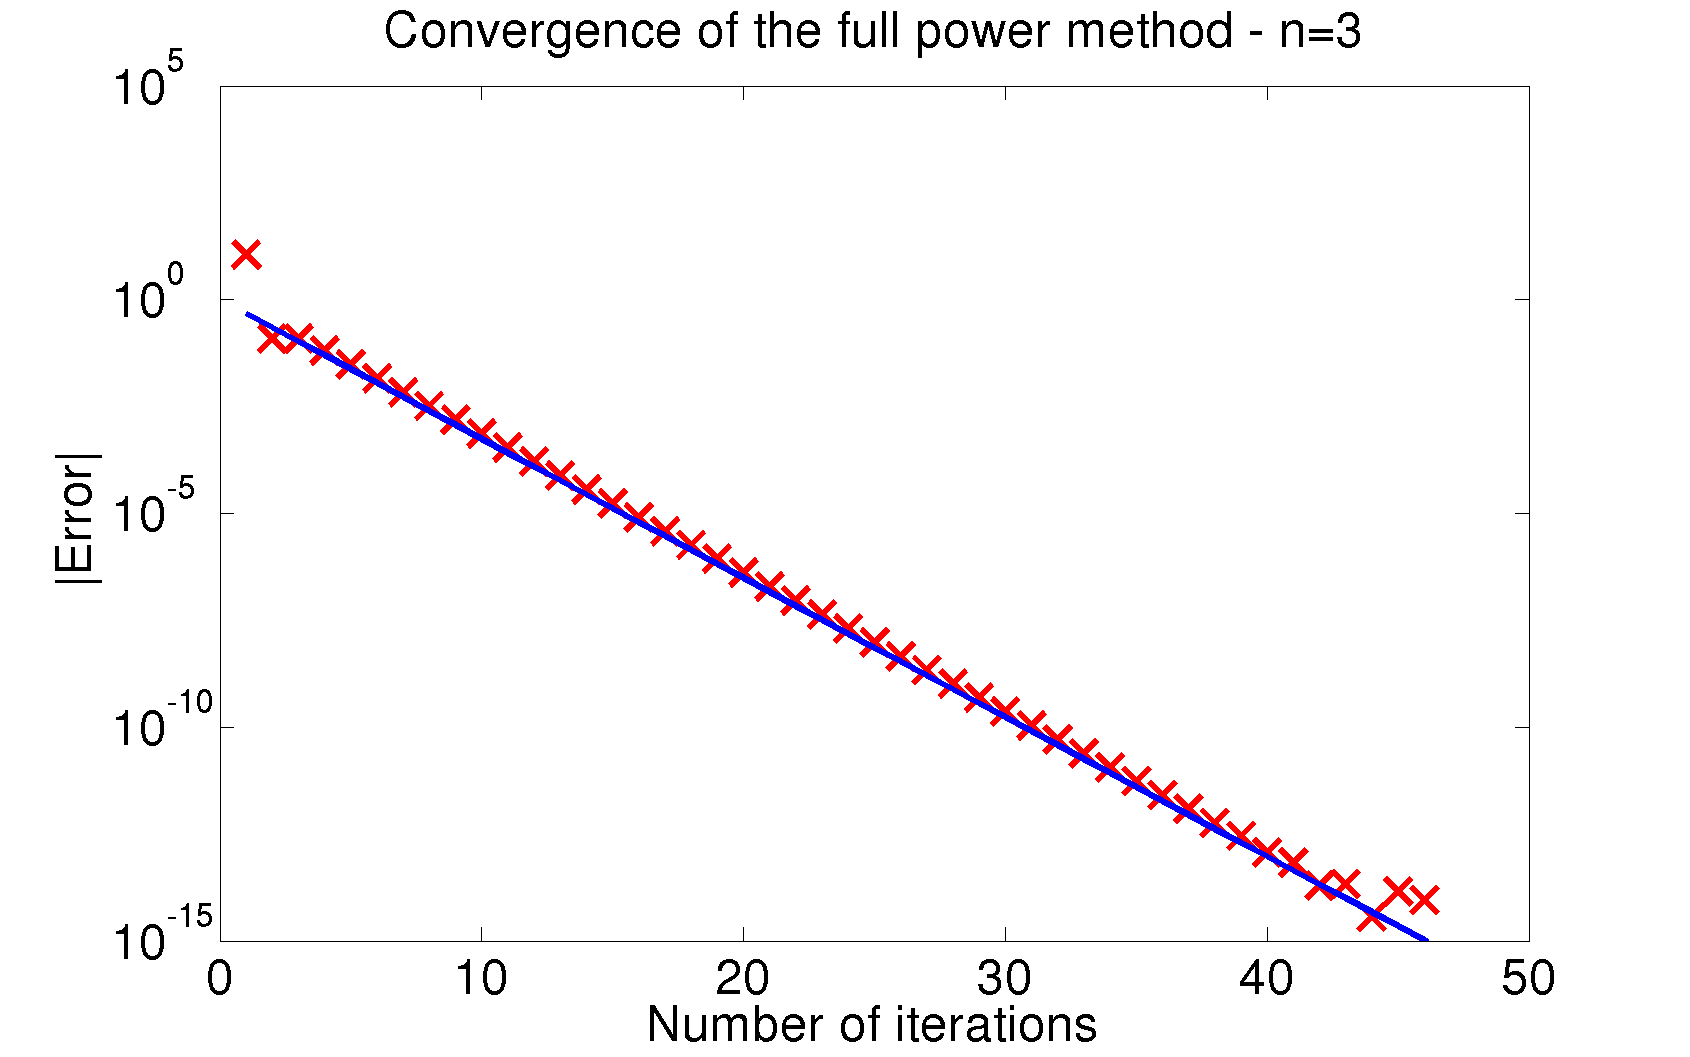
\includegraphics[width=\textwidth]{figures/PowerFull1}
    \end{column}
  \end{columns}
\end{frame}


\section{Summary}

\subsection{Summary}

\begin{frame}
  \frametitle{Summary}

  \begin{itemize}
  \item Eigenvalues of matrices contain fundamental information: we
    will frequently want or need to compute them. The eigenvalues of
    largest magnitude are frequently important for, e.g.\ the spectral
    radius.
  \item Computing the eigenvalues from the characteristic polynomial
    may be numerically ill-conditioned.
  \item The power method is an iterative scheme for finding the
    largest eigenvalue. It assumes that
    \begin{enumerate}
    \item There is a single largest eigenvalue;
    \item The eigenvectors are linearly independent.
    \end{enumerate}
  \item The power method converges linearly.
  \item The power method works when there are repeated eigenvalues;
    the eigenvector cannot be found, however. With distinct
    ``largest'' eigenvalues it may fail.
  \end{itemize}

\end{frame}

\end{document}



%%% Local Variables:
%%% mode: latex
%%% TeX-master: t
%%% End:
